\chapter{Flexion composée}
\section{Théorie}
	\subsection{Méthode cinématique}
	\begin{wrapfigure}[7]{r}{6.2cm}
	\vspace{-10mm}
	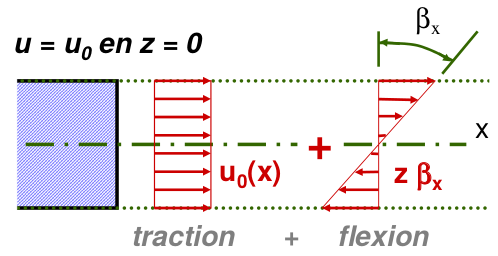
\includegraphics[scale=0.4]{ch7/image1.png}
	\captionof{figure}{ }
	\end{wrapfigure}
	On commence à connaître la chanson. Considérons une composition de ce qui a 
	été vu précédemment  un déplacement axial $u$ constant \textit{et} une 
	variation linéaire en fonction de la coordonnée Z.
	\begin{equation}
	u=u_0(x) + z\beta_x(x),\qquad v=0,\qquad w=w_0(x).
	\end{equation}
	Notons $O$, le centre géométrique.
	
	\subsection{Déplacements – Déformations – Contraintes}
		\subsubsection{Déformations}
		On combine : $\epsilon_x$ a une répartition constante \textit{et} est 
		linéaire en $z$ dans la section transversale 
		\begin{equation}
		\epsilon_x = \dfrac{\partial u_0}{\partial x}+z\dfrac{\partial\beta_x}{
		\partial x}
		\end{equation}
		On fait l'hypothèse que les sections planes restent planes ($\gamma_{xz}=\ 
		cste$) :
		\begin{equation}
		\gamma_{xz} = \beta_x+\dfrac{\partial w_0}{\partial x}
		\end{equation}
		
		\subsubsection{Contraintes}
		Toujours notre fameuse loi de Hooke, mais cette fois $\sigma_x$ a une 
		répartition constante \textit{et} une répartition linéaire en $z$ dans 
		la section transversale si $E$ est constant. Poisson encore et toujours 
		négligé. Par rapport à $\tau_{xz}$, cela dépend de si on tient compte 
		ou pas de l'hypothèse de Bernoulli.
		
	\subsection{Éléments de réduction : section constante}
	A l'aide de la loi de Hooke, nous avons
	\begin{equation}
	\begin{array}{ll}
	\sigma_x &=\displaystyle E\left(\dfrac{\partial u_0}{\partial x}+z\dfrac{
	\partial\beta_x}{\partial x}\right)\\
	&= \displaystyle \sigma_x^0 + Ez\dfrac{\partial\beta_x}{\partial x}
	\end{array}
	\end{equation}
	Calculons avant tout notre normale $N$
	\begin{equation}
	N = \int_A\sigma_x\ dA\qquad\ \Longrightarrow\qquad N = \sigma_x^0A
	\end{equation}
	En effet, $\sigma_x^0$ peut être sorti de l'intégrale, étant constant. 
	Comme on a fait dans les chapitres précédents, on suppose $\int_A z\ dA =0$ : 
	ceci est vrai si je passe par le centre géométrique de la figure. Le 
	raisonnement inverse est aussi acceptable : \textit{Cette condition doit 
	être vraie pour que mon effort normal ne dépende que de $\sigma$.}\\
	
	En faisant un raisonnement similaire pour $M_y$ :
	\begin{equation}
	M_y = \int_A \sigma_xz\ dA \qquad\Longrightarrow\qquad M_y = E\dfrac{
	\partial \beta_x}{\partial x}\int_A z^2\ dA
	\end{equation}
	Cette fois, le terme en $\sigma_c^0$ disparaît : car, encore, $\int_A z\ dA=0$.
	On a donc 
	\begin{equation}
	M_y = E\dfrac{\partial \beta_x}{\partial x}I_{zz}\qquad\text{ avec }\quad 
	I_{zz} = \int_A z^2\ dA
	\end{equation}		
	
		\subsubsection{En résumé}
		La poutre est soumise à un effort normal ($N$) \textit{et} à un moment 
		fléchissant ($M_y$). Comme nous avons :
		\begin{equation}
		\begin{array}{lll}
		\text{Pour la traction : } & \sigma_x^{(N)} &= \dfrac{N}{A}\\
		\text{Pour la flexion : } & \sigma_x^{(M)} &= \dfrac{M_y}{I_y}z		
		\end{array}
		\end{equation}
		On a donc
		\begin{equation}
		\sigma_x = \dfrac{N}{A}+\dfrac{M_y}{I_y}z
		\end{equation}
	
	
	
	
	
	
	
	
	
	
	
	
	
	
	
	
	